\chapter{Unsupervised Learning and Sequential Data Modelling – (Units 3 and 4)}

\section{Overview of Allotted Unit 3 and Unit 4 Topics}
Group 10's PBL II topic is \textbf{Sequential Human Activity Recognition}. The allotted algorithms are Markov models,
Hidden Markov Models (HMM), the forward–backward algorithm and the Viterbi algorithm. The objective is to infer
activity-state sequences from accelerometer time series.
\begin{itemize}
\item \textbf{Unit 3 (clustering and dimensionality reduction):} K-Means and Gaussian Mixture Model (GMM) clustering of
per-window accelerometer features, with PCA for visualisation. Clustering groups windows by similarity and ignores time
order, so it is the natural non-sequential baseline for the HMM.
\item \textbf{Unit 4 (sequential modelling):} a Gaussian HMM trained without labels (Baum–Welch), hand-implemented
forward–backward and Viterbi algorithms, and a supervised (hybrid) HMM that decodes the activity sequences of unseen
people.
\end{itemize}

\section{Unit 3 – Dataset Description and Preprocessing}
A new dataset is used for PBL II: the \textbf{UCI Human Activity Recognition Using Smartphones} dataset (UCI ML
Repository \#240) \cite{anguita}. Thirty volunteers aged 19–48 performed six activities (Walking, Walking
Upstairs, Walking Downstairs, Sitting, Standing, Laying) with a Samsung Galaxy S II worn on the waist.
\begin{itemize}
\item \textbf{Signal:} the triaxial accelerometer was sampled at \textbf{50 Hz}. The dataset authors pre-filtered the
signals and segmented them into \textbf{2.56 s windows} (128 samples) with 50\% overlap, giving \textbf{10,299 windows}.
\item \textbf{Size and balance:} classes are roughly balanced (Laying 1,944, Standing 1,906, Sitting 1,777,
Walking 1,722, Upstairs 1,544, Downstairs 1,406 windows). There are no missing values.
\item \textbf{Relevance:} the labels exist, but the unsupervised methods never use them for training; they serve only to
measure how well the hidden structure is recovered.
\end{itemize}
\textbf{Feature engineering.} Each window's raw signal ($128\times3$ total acceleration) is summarised into 10 features:
\begin{itemize}
\item the mean and standard deviation of the acceleration magnitude $\lVert\mathbf a\rVert$, and its energy;
\item the per-axis means (the direction of gravity, which encodes the phone's orientation);
\item the per-axis standard deviations;
\item the jerk energy (mean squared sample-to-sample difference).
\end{itemize}
Features are standardised with a scaler fitted on training subjects only.

\textbf{Split by person.} The data is split by subject: 24 subjects (8,013 windows) for training and 6 unseen subjects
(2,286 windows) for testing. Windows from the same person never appear in both sets.

\section{Unit 3 – Theory, EDA, Implementation and Results}
\begin{figure}[H]
\centering
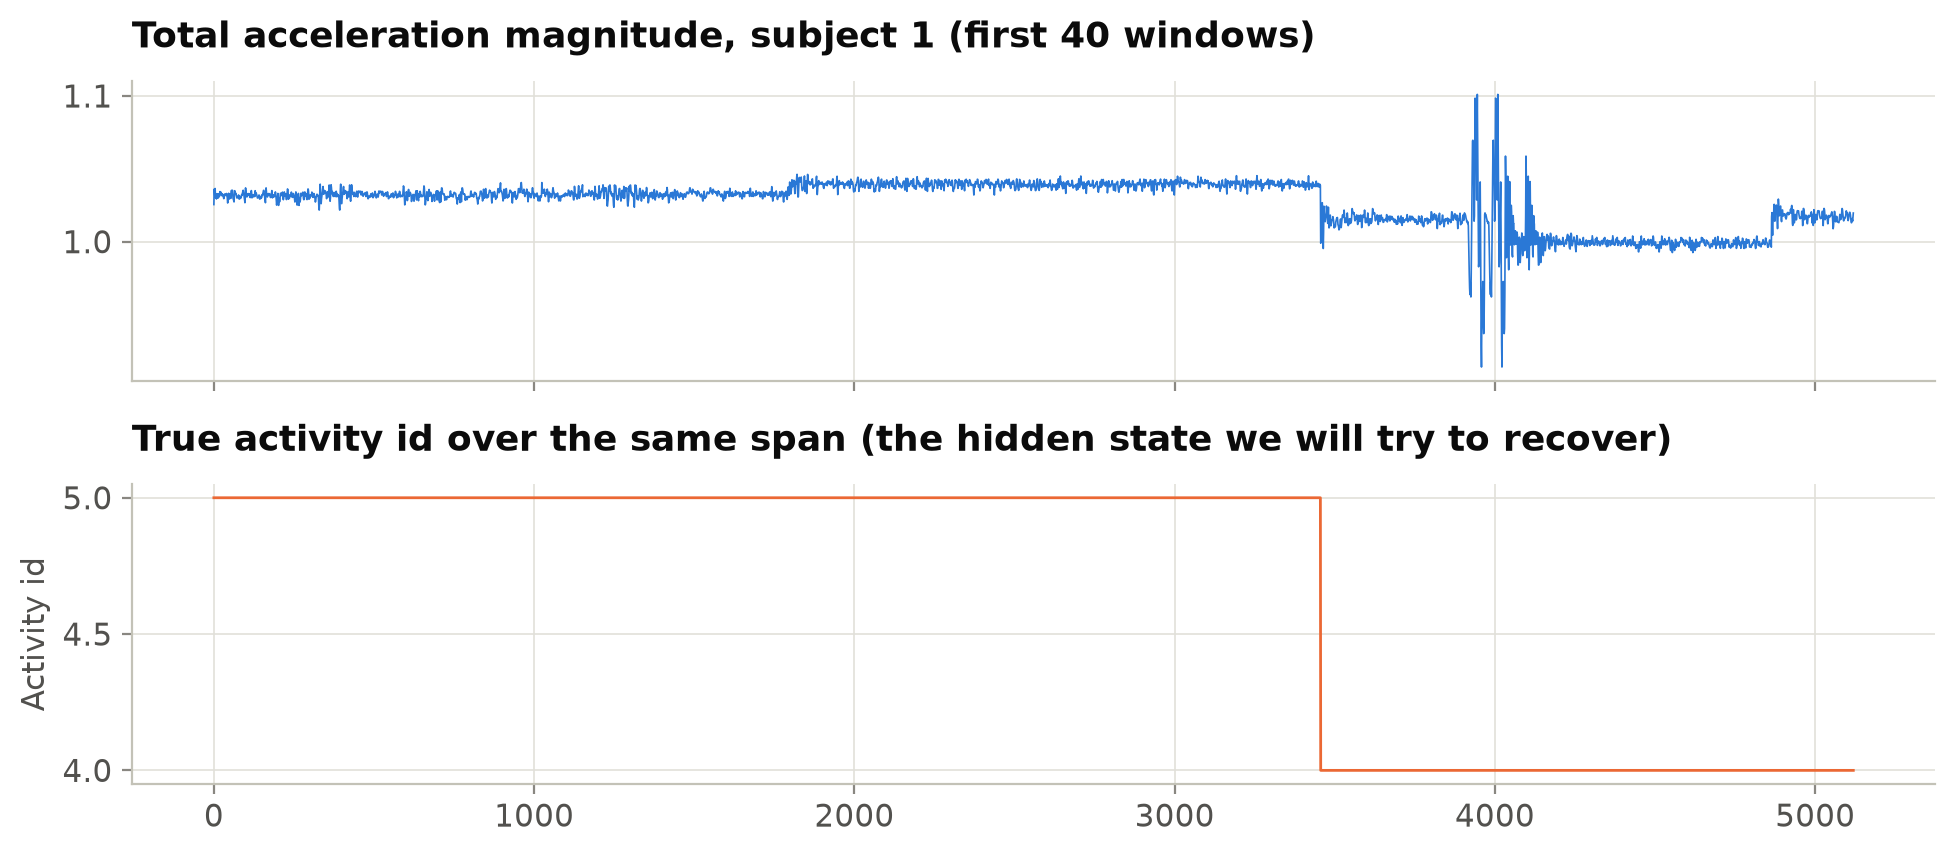
\includegraphics[width=0.53\linewidth]{har_signal_and_activity.png}\hfill
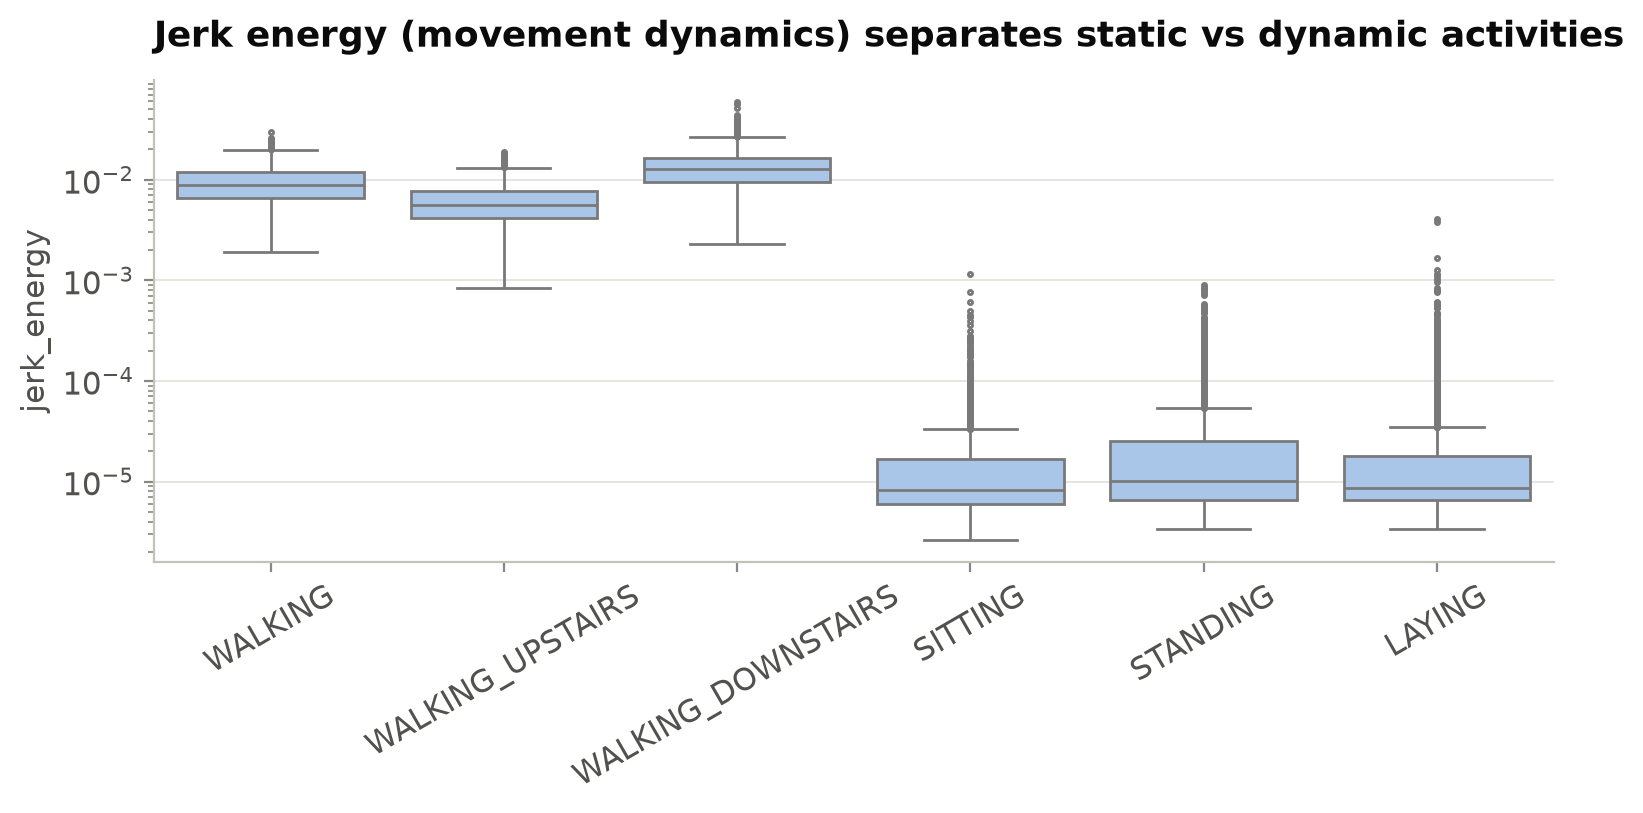
\includegraphics[width=0.45\linewidth]{har_jerk_by_activity.png}
\caption{HAR: acceleration magnitude and true activity for one subject (left); jerk energy by activity on a log scale (right)}
\label{fig:hareda}
\end{figure}
\textbf{Interpretation (Figure~\ref{fig:hareda}).} The acceleration magnitude stays near 1\,g (gravity) and is stable
while the activity is constant. It changes sharply when the activity switches: the burst near sample 3,500 is the act
of sitting down. Jerk energy separates \emph{dynamic} activities (about $10^{-2}$) from \emph{static} ones (about
$10^{-5}$), a thousand-fold gap. Within each group, however, the distributions overlap: Sitting, Standing and Laying look
alike, and so do the three walking types. The true activity is piecewise-constant, lasting on average
\textbf{29.5 windows ($\approx$38 s)} per bout. This persistence is the evidence for the Markov assumption.

\begin{figure}[H]
\centering
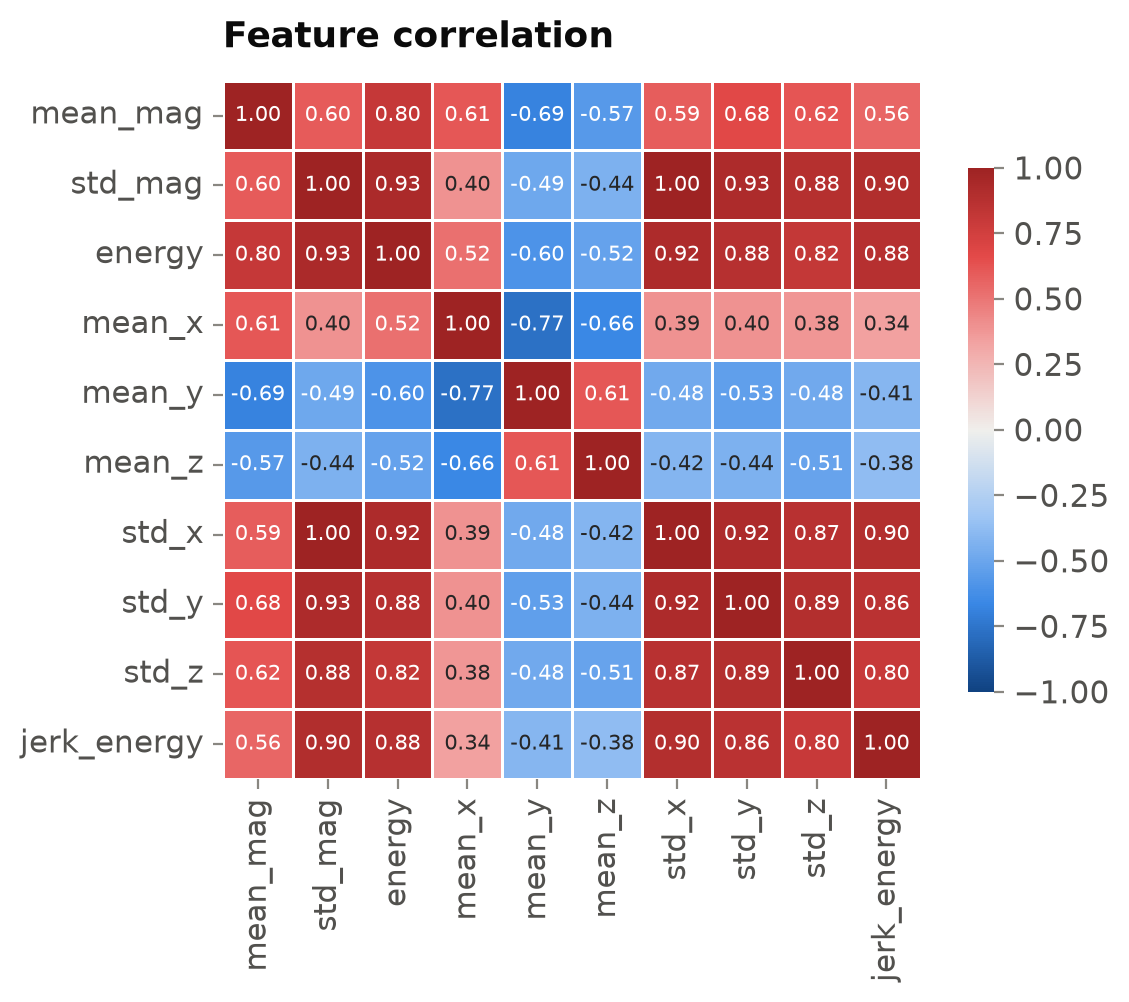
\includegraphics[width=0.62\linewidth]{har_feature_correlation.png}
\caption{Correlation between the ten engineered window features}
\label{fig:harcorr}
\end{figure}
\textbf{Interpretation (Figure~\ref{fig:harcorr}).} Magnitude statistics and per-axis standard deviations are strongly
correlated, so a few directions carry most of the information. This supports full-covariance Gaussian models (GMM and
HMM emissions), which capture the correlations, and a 2-D PCA projection for visualisation.

\section{Unit 3 – Algorithm Theory and Mathematical Formulation}
\textbf{K-Means} \cite{lloyd} partitions the windows $\{\mathbf x_i\}$ into $K$ clusters by minimising the within-cluster sum of
squares, alternating assignment and centroid update:
\begin{equation}
\min_{\{C_k\},\{\boldsymbol\mu_k\}}\ \sum_{k=1}^{K}\sum_{\mathbf x_i\in C_k}\lVert\mathbf x_i-\boldsymbol\mu_k\rVert^2 .
\end{equation}
\textbf{The Gaussian Mixture Model} is a soft, probabilistic generalisation fitted by Expectation–Maximisation \cite{dempster}:
\begin{equation}
p(\mathbf x)=\sum_{k=1}^{K}\pi_k\,\mathcal N(\mathbf x\mid\boldsymbol\mu_k,\boldsymbol\Sigma_k),\qquad
r_{ik}=\frac{\pi_k\,\mathcal N(\mathbf x_i\mid\boldsymbol\mu_k,\boldsymbol\Sigma_k)}{\sum_j\pi_j\,\mathcal N(\mathbf x_i\mid\boldsymbol\mu_j,\boldsymbol\Sigma_j)} .
\end{equation}
\textbf{PCA} projects the data onto the eigenvectors of its covariance matrix with the largest eigenvalues; it is used
only for 2-D visualisation. \textbf{Settings:} $K=6$ (one cluster per activity), K-Means with 10 restarts, GMM with full
covariances and 5 restarts. Clusters carry no names, so each cluster id is matched one-to-one to an activity by the
\textbf{Hungarian algorithm} \cite{kuhn} on the training confusion matrix, then applied unchanged to the test subjects.
\textbf{Metrics:} accuracy after matching; the Adjusted Rand Index (ARI, which needs no matching); the silhouette score;
and the average segment length (how many consecutive windows keep the same label).

\section{Unit 3 Proposed System Architecture / Workflow}
\begin{figure}[H]
\centering
\begin{tikzpicture}[node distance=0.4cm and 0.45cm, font=\small,
  box/.style={draw=navy, fill=lightblue, rounded corners=3pt, minimum height=1.1cm, text width=2.15cm, align=center},
  hl/.style={box, fill=lightorange, draw=accent}, arr/.style={-{Stealth[length=2.5mm]}, thick, navy}]
\node[box] (a) {Raw 50 Hz accelerometer};
\node[box, right=of a] (b) {2.56 s windows (128 samples)};
\node[box, right=of b] (c) {10 features per window};
\node[box, right=of c] (d) {Split by subject 24 / 6};
\node[box, below=0.9cm of d] (e) {Standardise (train only)};
\node[hl, left=of e] (f) {K-Means \& GMM ($K=6$)};
\node[box, left=of f] (g) {Hungarian cluster$\to$activity};
\node[hl, left=of g] (h) {Accuracy, ARI, silhouette, PCA view};
\draw[arr] (a)--(b); \draw[arr] (b)--(c); \draw[arr] (c)--(d); \draw[arr] (d)--(e);
\draw[arr] (e)--(f); \draw[arr] (f)--(g); \draw[arr] (g)--(h);
\end{tikzpicture}
\caption{Unit 3 clustering workflow}
\label{fig:wf3}
\end{figure}
The raw signal is cut into windows and summarised as features. The data is split by subject, and the features are
standardised on the training subjects. K-Means and GMM cluster the training windows. The Hungarian algorithm gives the
clusters activity names, and evaluation happens on the six unseen subjects.

\section{Unit 3 – Results and Performance Evaluation}
\begin{figure}[H]
\centering
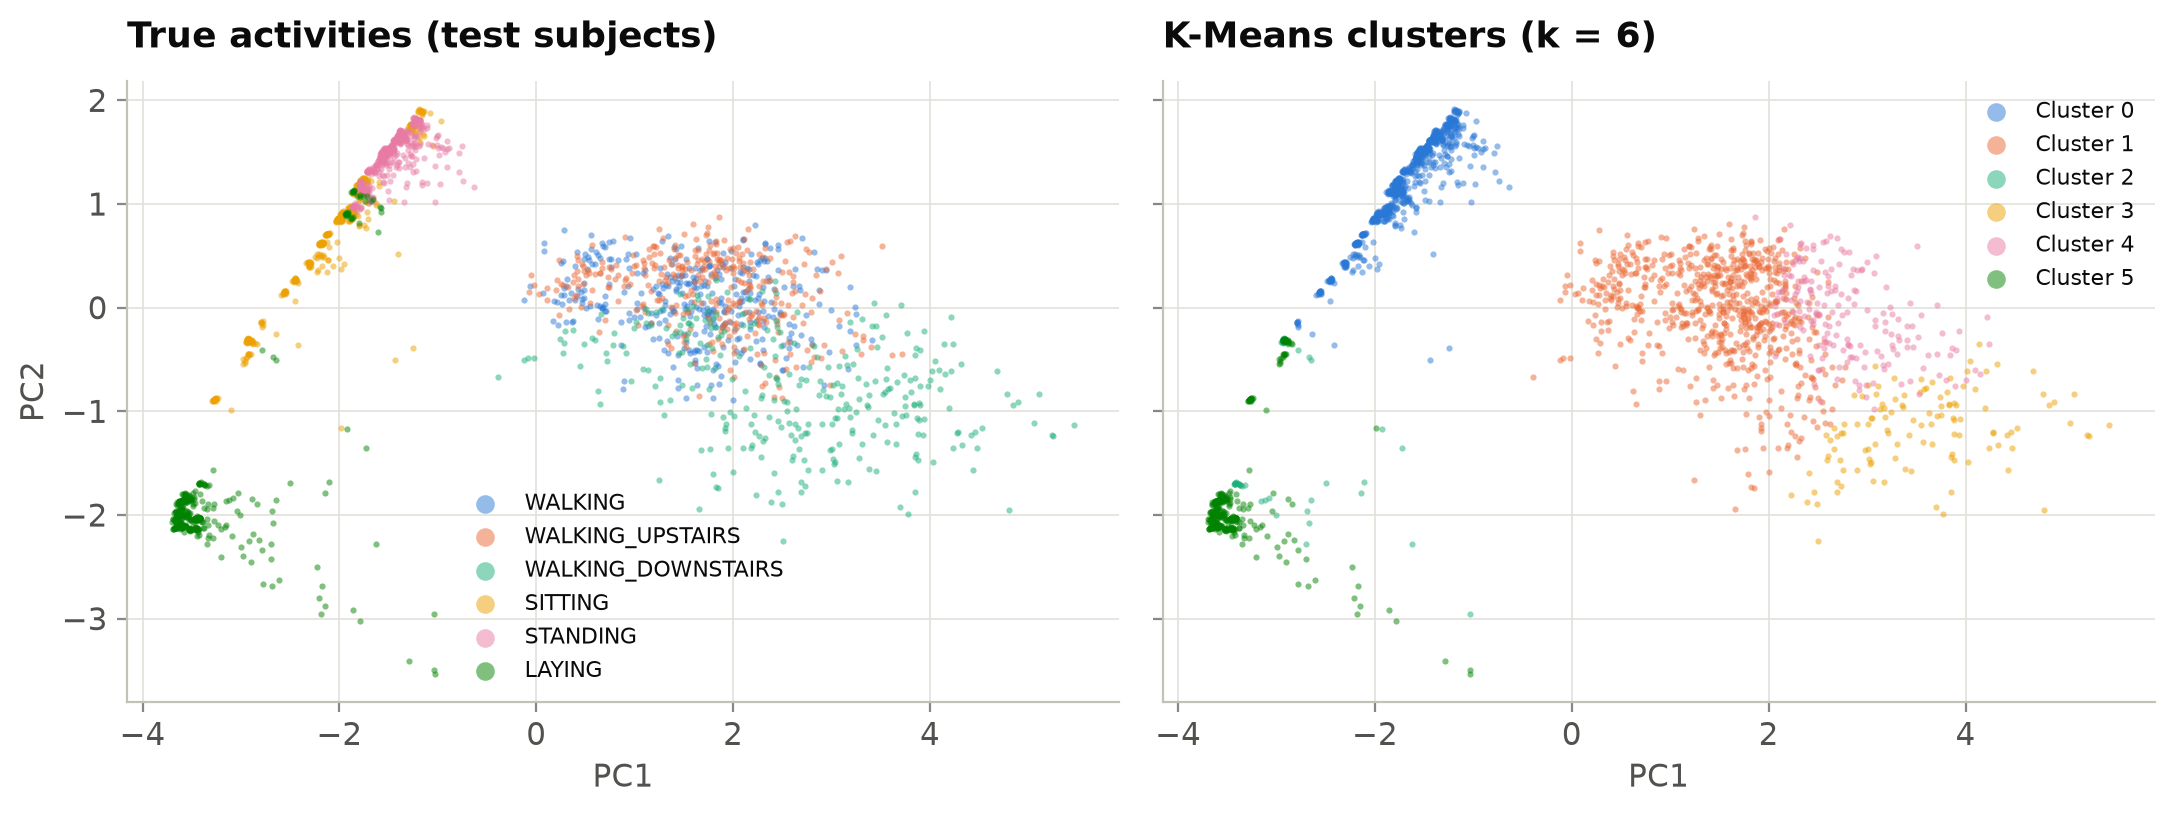
\includegraphics[width=0.92\linewidth]{har_pca_clusters.png}
\caption{Test windows in PCA space, coloured by true activity (left) and by K-Means cluster (right)}
\label{fig:harpca}
\end{figure}
\begin{table}[H]
\centering
\caption{Unit 3: clustering results on the six unseen test subjects}
\label{tab:unit3}
\begin{tabular}{@{}lcccc@{}}
\toprule
\textbf{Method} & \textbf{Accuracy} & \textbf{ARI} & \textbf{Silhouette} & \textbf{Avg segment (windows)} \\
\midrule
K-Means ($K=6$) & 0.570 & 0.464 & 0.412 & 7.8 \\
Gaussian Mixture ($K=6$) & 0.612 & 0.486 & 0.357 & 11.1 \\
True activity labels & 1.000 & 1.000 & 0.257 & 29.5 \\
\bottomrule
\end{tabular}
\end{table}
\textbf{Interpretation (Figure~\ref{fig:harpca}, Table~\ref{tab:unit3}).} Clustering recovers the coarse structure.
Laying forms its own tight cluster, and the dynamic activities form a separate cloud. GMM reaches 61.2\% accuracy and
K-Means 57.0\%; random guessing over six classes would give 16.7\%. K-Means merges Sitting and Standing into one cluster
and splits the walking cloud along boundaries that do not match Walking, Upstairs and Downstairs. Interestingly, the
clusters have a \emph{higher} silhouette than the true labels (0.41 vs 0.26): the geometric ``natural groups'' in feature
space are not the same as the semantic activities. Clustering also ignores time, so its labels flicker, with segments of
only 7.8–11.1 windows against 29.5 in reality.

\section{Unit 4 – Sequential Dataset Description}
Unit 4 uses the same UCI HAR recordings, treated as \textbf{time series}:
\begin{itemize}
\item \textbf{Sequence identifier:} the subject id. Each subject's windows form one continuous, time-ordered sequence
(30 sequences; the six test sequences contain 2,286 windows in total).
\item \textbf{Sampling:} 50 Hz raw signal; one observation per 2.56 s window, with a 1.28 s step.
\item \textbf{Hidden state:} the activity in each window ($S=6$ states). \textbf{Observation:} the 10 engineered
features (unsupervised HMM), or the dataset's 561 accelerometer and gyroscope features (supervised HMM).
\item \textbf{Data quality:} there are no missing windows. \textbf{Limitation:} the data was recorded in a laboratory
protocol with a fixed waist-worn phone position.
\end{itemize}

\section{Unit 4 – Sequential Preprocessing and EDA}
Temporal order is preserved throughout. Rows are sorted by subject with a \emph{stable} sort, so the original time order
within each subject is kept, and each subject is passed to the model as a separate sequence. States therefore never
carry over from one person to the next. Scalers are fitted on the training subjects only. The EDA in
Figure~\ref{fig:hareda} shows that activities persist for long bouts and that the signal changes at bout boundaries.
Both properties are exactly what a first-order Markov chain of hidden states with state-dependent emissions describes.

\section{Unit 4 – Mathematical Formulation}
An HMM $\lambda=(\boldsymbol\pi,\mathbf A,\mathbf B)$ over hidden states $s_t\in\{1,\dots,S\}$ and observations
$\mathbf x_t$ is defined by \cite{rabiner,murphy}:
\begin{equation}
\pi_i=P(s_1=i),\qquad a_{ij}=P(s_{t+1}=j\mid s_t=i),\qquad b_j(\mathbf x_t)=\mathcal N(\mathbf x_t\mid\boldsymbol\mu_j,\boldsymbol\Sigma_j).
\end{equation}
The Markov assumption is that $s_{t+1}$ depends only on $s_t$. The \textbf{forward} and \textbf{backward} recursions are
\begin{equation}
\alpha_t(j)=b_j(\mathbf x_t)\sum_{i}\alpha_{t-1}(i)\,a_{ij},\qquad
\beta_t(i)=\sum_{j}a_{ij}\,b_j(\mathbf x_{t+1})\,\beta_{t+1}(j),
\end{equation}
and their product gives the posterior state probability used for ``most likely state per window'' decoding:
\begin{equation}
\gamma_t(i)=P(s_t=i\mid\mathbf x_{1:T})=\frac{\alpha_t(i)\beta_t(i)}{\sum_j\alpha_t(j)\beta_t(j)} .
\end{equation}
\textbf{Viterbi} \cite{viterbi} finds the single most likely state sequence by dynamic programming, with back-pointers $\psi_t$:
\begin{equation}
\delta_t(j)=\max_i\big[\delta_{t-1}(i)+\log a_{ij}\big]+\log b_j(\mathbf x_t),\qquad
\psi_t(j)=\arg\max_i\big[\delta_{t-1}(i)+\log a_{ij}\big].
\end{equation}
\textbf{Unsupervised training} uses Baum–Welch (EM) \cite{baum}. It re-estimates, for example,
$a_{ij}=\sum_t\xi_t(i,j)/\sum_t\gamma_t(i)$, where $\xi_t(i,j)$ is the posterior probability of the transition
$i\to j$. \textbf{Supervised training} estimates the Markov chain by counting (maximum likelihood, +1 smoothing):
$a_{ij}=(n_{ij}+1)/\sum_k(n_{ik}+1)$. In the \textbf{hybrid HMM} the emission is a classifier's posterior divided by the
class prior, a scaled likelihood \cite{bourlard}: $b_j(\mathbf x)\propto P(s=j\mid\mathbf x)/P(s=j)$. All recursions are computed in log
space or with per-step scaling to avoid numerical underflow.

\section{Unit 4 Proposed System Architecture / Workflow}
\begin{figure}[H]
\centering
\begin{tikzpicture}[node distance=0.4cm and 0.45cm, font=\small,
  box/.style={draw=navy, fill=lightblue, rounded corners=3pt, minimum height=1.1cm, text width=2.2cm, align=center},
  hl/.style={box, fill=lightorange, draw=accent}, arr/.style={-{Stealth[length=2.5mm]}, thick, navy}]
\node[box] (a) {Per-subject ordered sequences};
\node[box, right=of a] (b) {Features: 10 (unsup.) / 561 (sup.)};
\node[hl, above right=0.15cm and 0.45cm of b] (c) {Baum–Welch EM (no labels)};
\node[hl, below right=0.15cm and 0.45cm of b] (d) {Count $\mathbf A,\boldsymbol\pi$ + classifier emissions};
\node[box, right=2.9cm of b] (e) {Forward–backward \& Viterbi (hand-coded)};
\node[box, right=of e] (f) {Decoded activity sequence};
\node[box, below=0.9cm of f] (g) {Accuracy, F1, ARI, segment length};
\draw[arr] (a)--(b); \draw[arr] (b)--(c); \draw[arr] (b)--(d); \draw[arr] (c)--(e); \draw[arr] (d)--(e);
\draw[arr] (e)--(f); \draw[arr] (f)--(g);
\end{tikzpicture}
\caption{Unit 4 sequential modelling workflow (unsupervised and supervised HMM)}
\label{fig:wf4}
\end{figure}
Each subject's windows form one ordered sequence. In the \emph{unsupervised} path, Baum–Welch learns
$(\boldsymbol\pi,\mathbf A,\mathbf B)$ from the 10 features without labels: 6 states, full-covariance Gaussian emissions,
8 random restarts. In the \emph{supervised} path, $\mathbf A$ and $\boldsymbol\pi$ are counted from labelled training
sequences, and the emissions come from either an LDA classifier (one Gaussian per activity) or a logistic-regression
classifier (hybrid HMM) on the 561 features. Both paths decode each test subject with our own forward–backward and
Viterbi implementations.

\section{Results and Performance Evaluation}
\textbf{Verification of the hand-coded algorithms.} On a test subject, our forward–backward posteriors match
\texttt{hmmlearn}'s \texttt{predict\_proba} to within $1.5\times10^{-10}$, and our Viterbi path is identical to
\texttt{hmmlearn.predict}.

\begin{figure}[H]
\centering
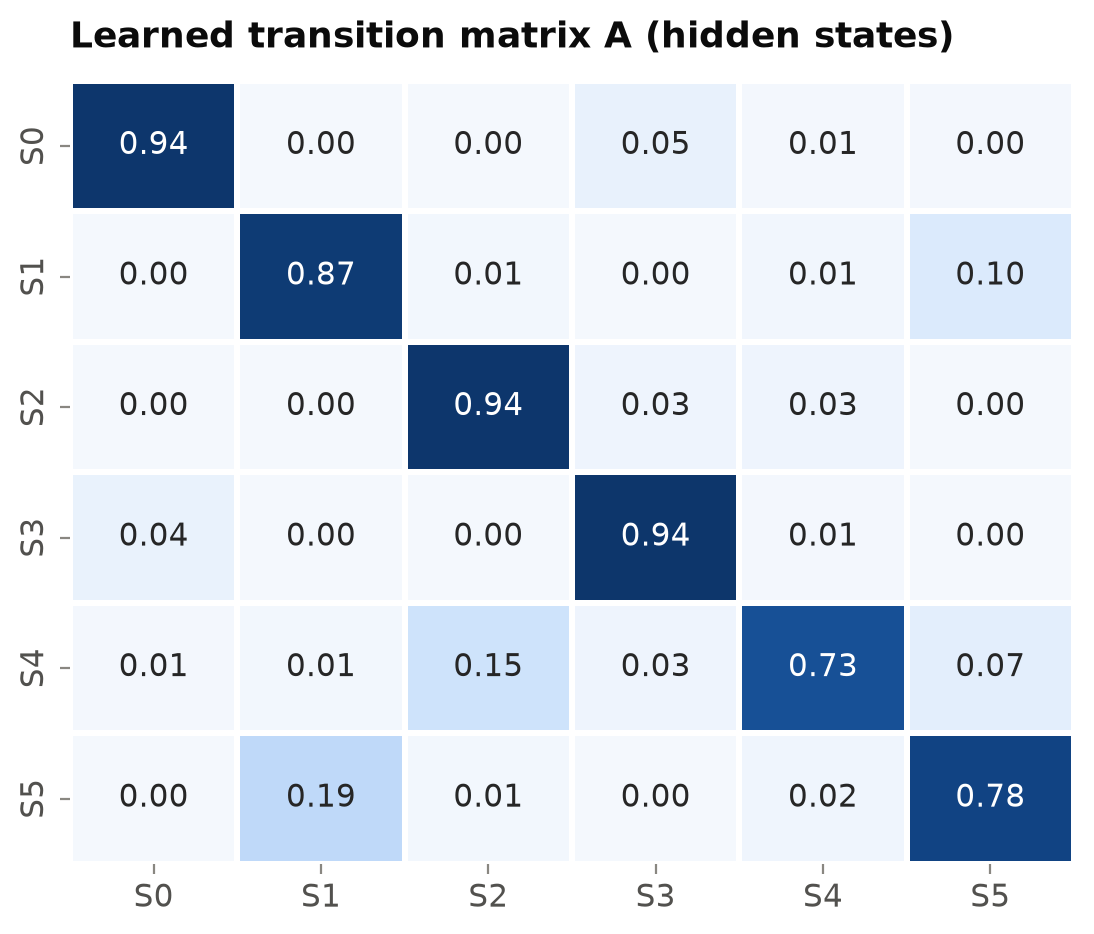
\includegraphics[width=0.40\linewidth]{har_transition_matrix.png}\hfill
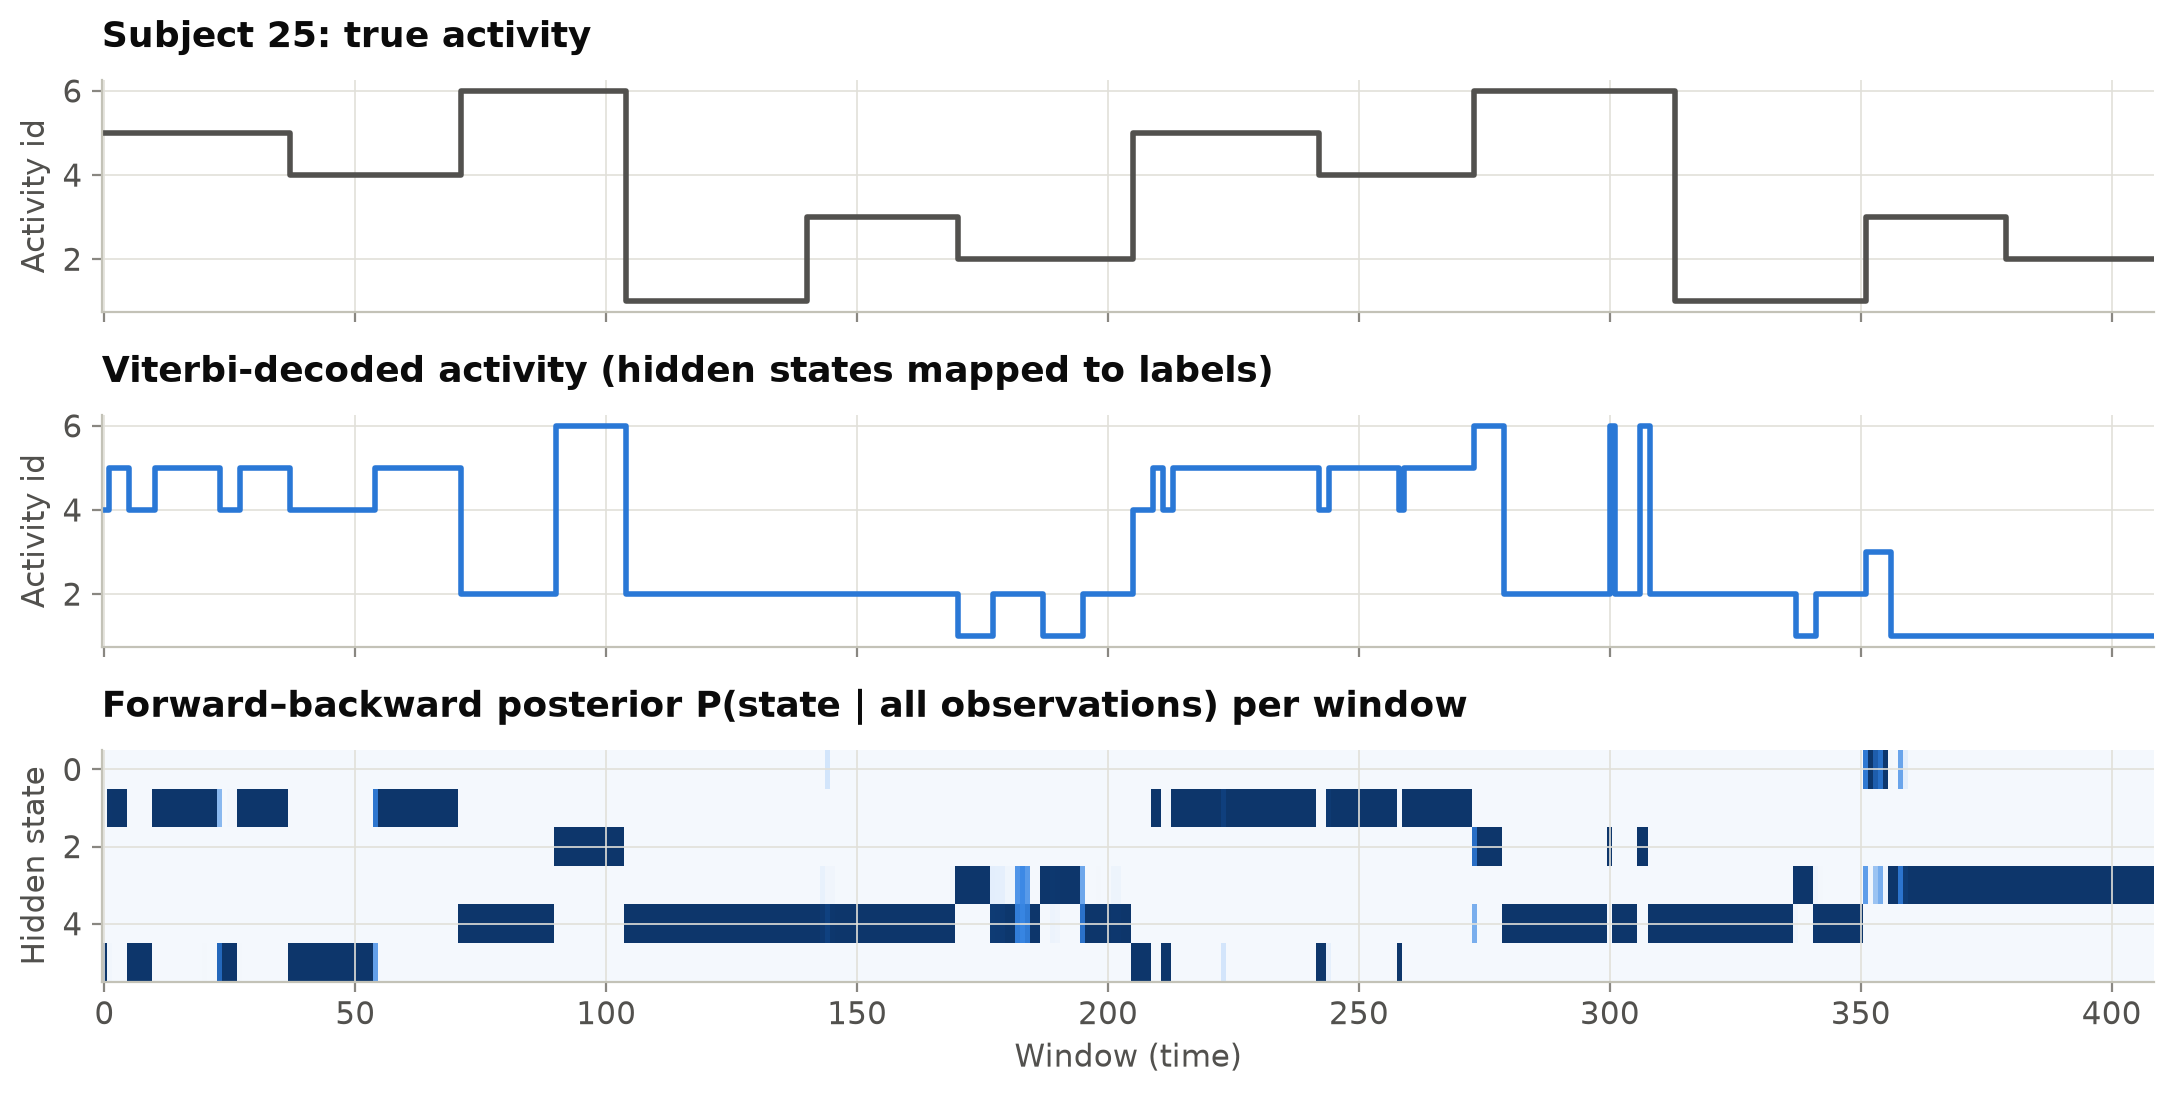
\includegraphics[width=0.58\linewidth]{har_decoded_timeline.png}
\caption{Unsupervised HMM: learned transition matrix (left); true vs Viterbi-decoded activities and forward–backward posteriors for test subject 25 (right)}
\label{fig:hmmunsup}
\end{figure}
\textbf{Interpretation (Figure~\ref{fig:hmmunsup}).} Without any labels, the HMM learns a strongly diagonal transition
matrix (0.73–0.94): states persist, as real activities do. The forward–backward posteriors are confident (near 0 or 1)
and switch exactly where the true activity changes, so the model detects \emph{when} transitions happen.

\begin{table}[H]
\centering
\caption{Unit 4: sequence decoding on the six unseen test subjects (2,286 windows)}
\label{tab:unit4}
\begin{tabular}{@{}llccc@{}}
\toprule
\textbf{Model} & \textbf{Decoding} & \textbf{Accuracy} & \textbf{Macro F1} & \textbf{Avg segment} \\
\midrule
Unsupervised Gaussian HMM (10 features) & Viterbi & 0.598 & – & 11.7 \\
LDA emissions (561 features) & per window, no HMM & 0.968 & 0.967 & 18.5 \\
LDA emissions + HMM & Viterbi & 0.975 & 0.974 & 25.6 \\
Logistic-regression emissions & per window, no HMM & 0.964 & 0.966 & 15.9 \\
\rowcolor{lightorange} Hybrid HMM (logistic regression) & Viterbi & \textbf{0.987} & \textbf{0.988} & 27.4 \\
Hybrid HMM (logistic regression) & forward–backward & 0.987 & 0.988 & 27.4 \\
\midrule
True activity sequence & – & 1.000 & 1.000 & 29.5 \\
\bottomrule
\end{tabular}
\end{table}
\begin{figure}[H]
\centering
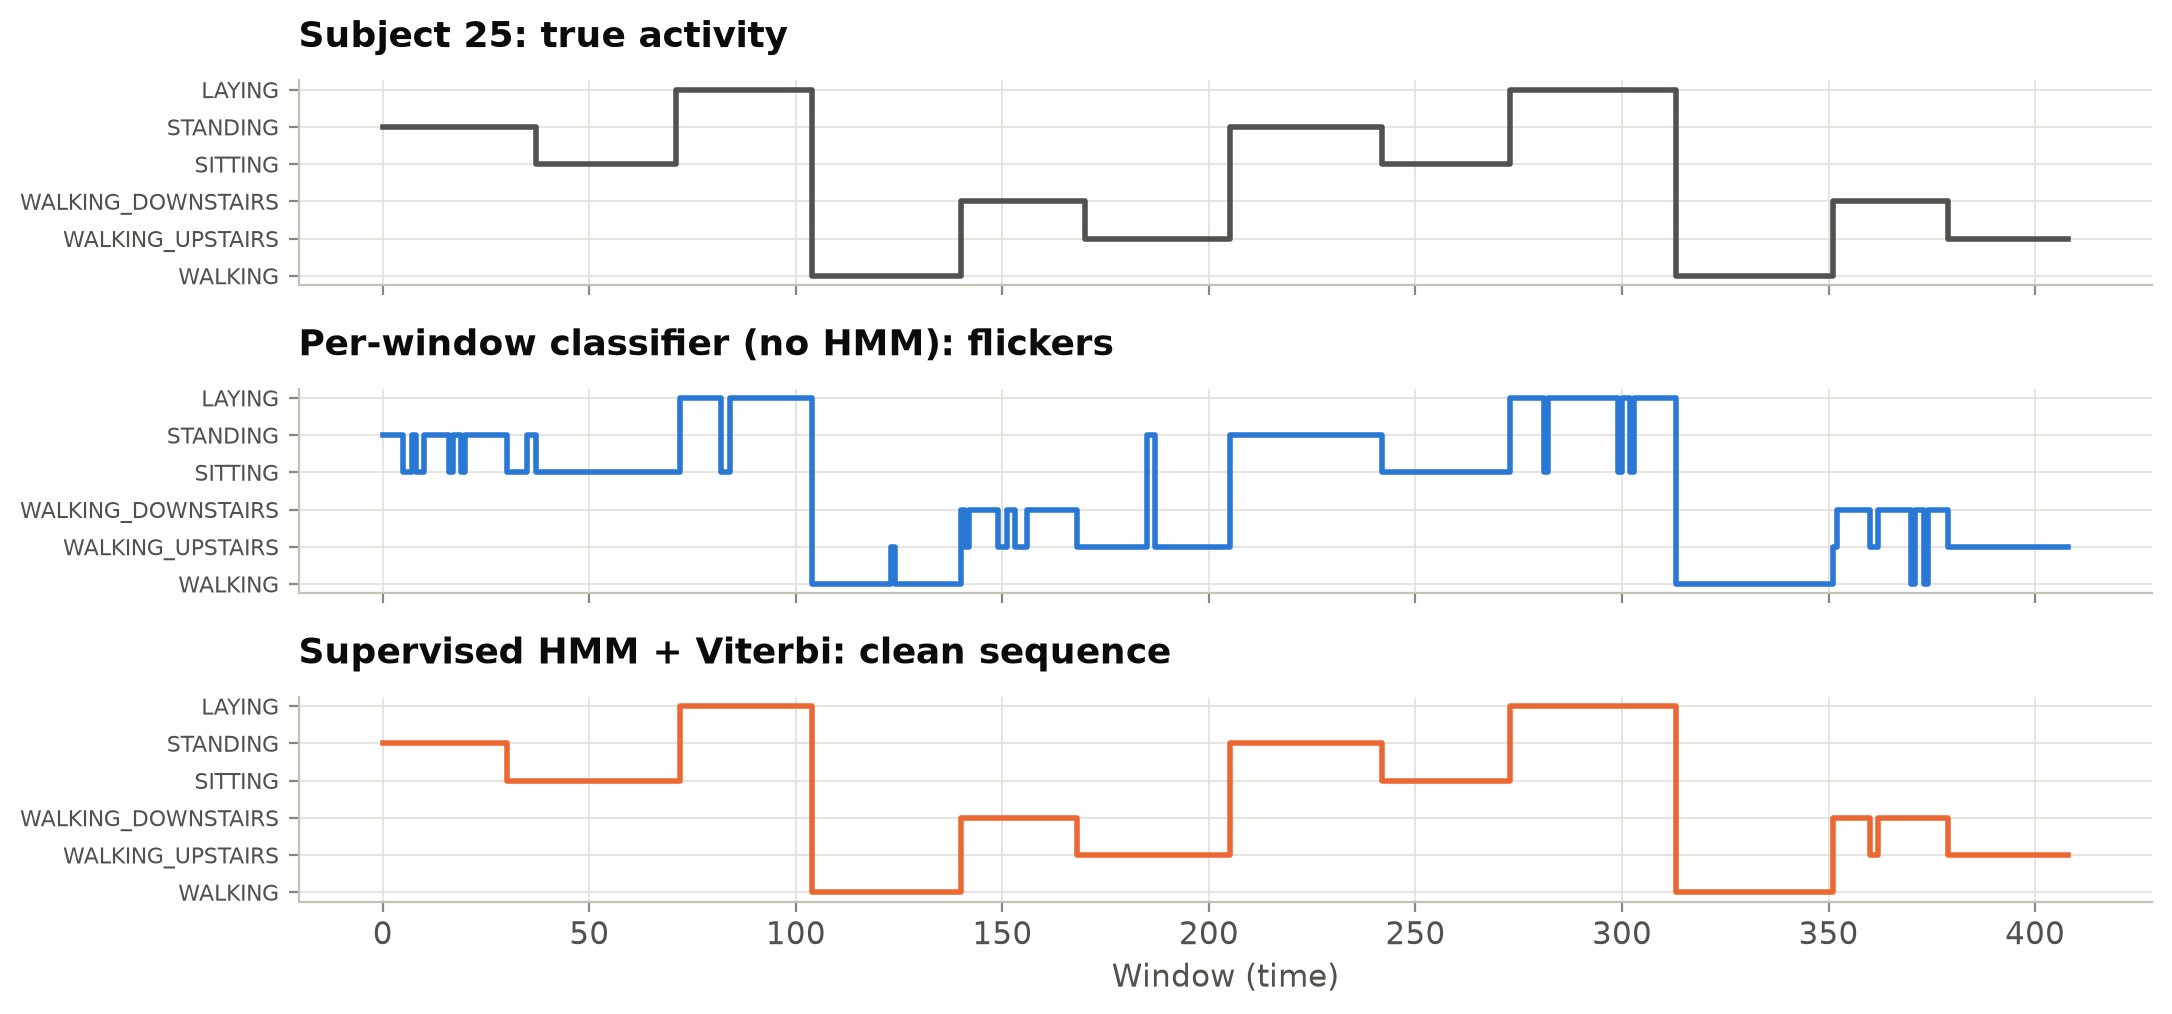
\includegraphics[width=0.56\linewidth]{har_supervised_timeline.png}\hfill
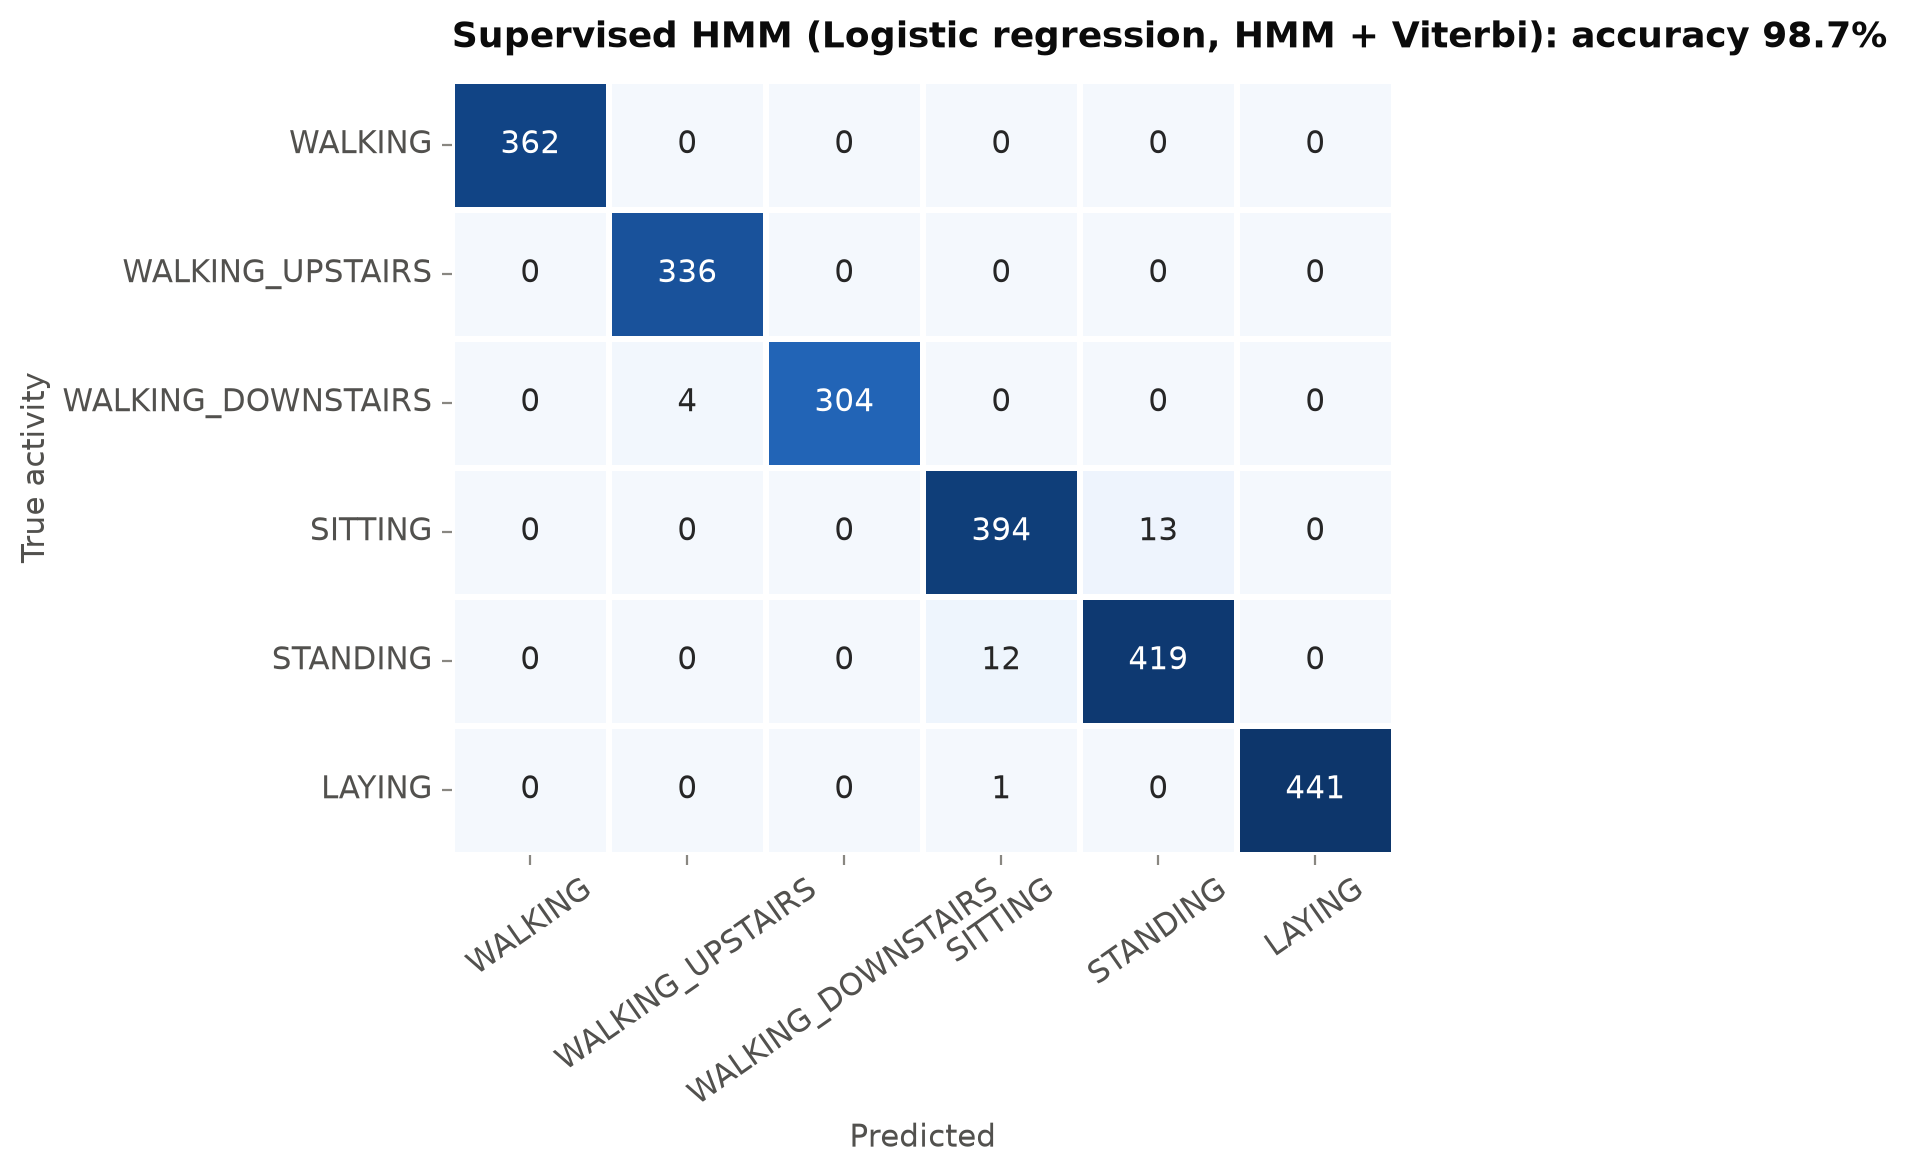
\includegraphics[width=0.42\linewidth]{har_confusion_supervised.png}
\caption{Supervised hybrid HMM: per-window classifier vs HMM + Viterbi for subject 25 (left); test confusion matrix (right)}
\label{fig:hmmsup}
\end{figure}
\textbf{Interpretation (Table~\ref{tab:unit4}, Figure~\ref{fig:hmmsup}).} The supervised hybrid HMM decodes the activities
of unseen people with \textbf{98.7\% accuracy} (macro F1 0.988). Holding the classifier fixed, adding the Markov chain
with Viterbi raises accuracy from 96.4\% to 98.7\%, removing \textbf{63\% of the errors}. It also lengthens the decoded
bouts from 15.9 to 27.4 windows, close to the true 29.5: Viterbi suppresses isolated one-window flickers that contradict
the surrounding activity. Walking and Walking Upstairs, the pair the unsupervised model confused most, are now classified
perfectly (362/362 and 336/336). Only 30 of 2,286 windows are wrong, and 25 of those are Sitting $\leftrightarrow$
Standing.

\section{Discussion, Findings and Limitations}
\begin{itemize}
\item \textbf{Clustering (Unit 3)} finds the geometric structure of the data but not the semantic activities. Similar
activities overlap in feature space, and time order is ignored.
\item \textbf{The unsupervised HMM} adds temporal consistency (segments of 11.7 vs 7.8 windows for K-Means) but no
accuracy gain (59.8\%). Its states must be discovered blindly from 10 accelerometer features, which cannot separate
stairs from walking or sitting from standing.
\item \textbf{The supervised HMM} shows the real value of sequential modelling. The Markov transition structure corrects
most of the remaining mistakes of a strong per-window classifier.
\item \textbf{State definitions and validation:} each state is defined as one activity. This is reasonable, but a
multi-state-per-activity or semi-Markov (explicit duration) model could represent within-activity dynamics better.
Validation is by unseen \emph{subjects}, the appropriate test of generalisation for sequential data.
\item \textbf{Limitations:} laboratory protocol, a fixed phone position, and only six test subjects.
\end{itemize}

\section{Chapter Conclusion}
Unit 3 showed that unsupervised clustering recovers the coarse static/dynamic structure of activity data (accuracy
57–61\%) but cannot label activities reliably. Unit 4 implemented and verified forward–backward and Viterbi, showed that
an unsupervised HMM learns realistic persistence without labels, and reached \textbf{98.7\% accuracy on unseen people}
with a supervised hybrid HMM. Its Markov chain removes 63\% of a per-window classifier's errors. These results are on a
different dataset from Units 1, 2 and 5, so they are not compared numerically with the other chapters.
